\documentclass{ctuthesis}

\ctusetup{
    xdoctype = B,
    xfaculty = F3,
    mainlanguage = czech,
    secondlanguage = english,
    titlelanguage = czech,
    title-english = {UI toolkit of accessible web components},
    title-czech = {UI toolkit přístupných webových komponent},
    department-czech = {Katedra počítačové grafiky a interakce},
    department-english = {Department of Computer Graphics and Interaction},
    fieldofstudy-czech = {Softwarové inženýrství a technologie},
    subfieldofstudy-czech = {Programátor / architekt webových aplikací},
    keywords-czech={Web komponenty, přístupnost, WAI-ARIA, WCAG, APG, Solid.js},
    keywords-english={Web components, accessibility, WAI-ARIA, WCAG, APG, Solid.js},
    author = {Pavel Sušický},
    supervisor = {Bc. Petr Huřťák},
    month = 5,
    year = 2024,
    specification-file={./assets/documents/zadani.pdf},
    front-specification={true}
}

\usepackage{csquotes,pdflscape,enumitem}
\usepackage[export]{adjustbox}

\usepackage[style=numeric,backend=biber,sorting=none]{biblatex}

\addbibresource{thesis.bib}

\usepackage[style=altlist]{glossaries}

\makenoidxglossaries{}

\newacronym{wcag}{WCAG}{Web Content Accessibility Guidelines}
\newacronym{waiaria}{WAI-ARIA}{Web Accessibility Initiative --- Accessible Rich Internet Applications}
\newacronym{apg}{APG}{ARIA Authoring Practices Guide}
\newacronym{w3c}{W3C}{World Wide Web Consortium}
\newacronym{wai}{WAI}{Web Accessibility Initiative}

\newacronym{dom}{DOM}{Document Object Model}
\newacronym{vdom}{VDOM}{Virtual DOM}

\newglossaryentry{lighthouse}{
    name={Ligthouse},
    description={Lighthouse je nástroj od Google pro provádění auditu stránky z různých hledisek. V kontextu této práce je využivána ``Time To Interactive'' metrika a velikost přenesených dat},
}

\newglossaryentry{todomvc}{
    name={TodoMVC},
    description={TodoMVC je kolekce příkladové aplikace implementované v různých webových technologiích},
}

\begin{listing}
    \begin{minted}{jsx}
const Toolbar: VoidComponent<Props> = (props) => {
    let toolbar;

    const {
        toolbarProps
    } = createToolbar(props, () => toolbar);

    return (
        <div ref={toolbar} {...toolbarProps}>
            <button onClick={() => alert("Bold")}>
                Bold
            </button>

            <button onClick={() => alert("Italics")}>
                Italics
            </button>
        </div>
    );
};
\end{minted}
    \caption{Ukázka použití createToolbar funkce}
    \label{toolbar-example}
\end{listing}

\begin{listing}
    \begin{minted}{jsx}
const Tooltip = (props) => {
    const [local, rest] = splitProps(props, ["state"]);
    const { tooltipProps } = createTooltip(props, () => local.state);
    
    return (
        <div {...tooltipProps}>{props.children}</div>
    );
};

export const TooltipTrigger = (props) => {
    let trigger;
    
    const state = createTooltipTriggerState(props);
    const {
        tooltipProps,
        triggerProps
    } = createTooltipTrigger(props, state, () => trigger);
    
    return (
        <button ref={trigger} {...triggerProps}>
            Hover or Focus me
            {state.isOpen ? (
                <Tooltip {...tooltipProps} state={state}>
                    {props.children}
                </Tooltip>
            ) : null}
        </button>
    );
};
\end{minted}
    \caption{Ukázka vytvoření Tooltipu}
    \label{tooltip-example}
\end{listing}

\begin{listing}
    \begin{minted}{jsx}
const Disclosure: VoidComponent<Props> = (props) => {
    const {
        toggleProps,
        contentProps,
        state
    } = createDisclosure(props);

    return (
        <div>
            <button {...toggleProps}>Toggle</button>
            {state.isVisible ? (
                <div {...contentProps}>
                    {props.children}
                </div>
            ) : null}
        </div>
    );
};
\end{minted}
    \caption{Ukázka použití createDisclosure funkce}
    \label{disclosure-example}
\end{listing}

\begin{listing}
    \begin{minted}{jsx}
const SpinButton: VoidComponent<Props> = () => {
    const { 
        inputProps,
        incrementButtonProps,
        decrementButtonProps,
        state
    } = createSpinButton({
        values: [1, 2, 3, 4, 5, 6, 7],
        mapping: [
            "monday",
            "tuesday",
            "wednesday",
            "thursday",
            "friday",
            "saturday",
            "sunday"
        ],
        step: 2
    });

    return (
        <div>
            <button {...incrementButtonProps}>up</button>
            <input {...inputProps} value={state.value} />
            <button {...decrementButtonProps}>down</button>
        </div>
    );
};
\end{minted}
    \caption{Ukázka použití createSpinButton funkce}
    \label{spinbutton-example}
\end{listing}

\begin{listing}
    \begin{minted}{markdown}
---!\mintedlabel{docs-page-example-1}!
title: Toolbar
description: a primitive for creating a Toolbar component
sidebar:
    badge:
        text: v0
        variant: success
---!\mintedlabel{docs-page-example-8}!

<Links github="https://example.com" />!\mintedlabel{docs-page-example-10}!

## Anatomy

<Anatomy viewBox="0 0 64 64" alt="0" caption="Example">
    <ToolbarAnatomy />
</Anatomy>

## API Reference

<PropTable name="ToolbarArguments" />!\mintedlabel{docs-page-example-20}!

## Example

<Toolbar client:idle />!\mintedlabel{docs-page-example-24}!
\end{minted}
    \caption{Ukázka stránky dokumentace psané v MDX}
    \label{docs-page-example}
\end{listing}

\begin{table}[ht]
    \begin{tabularx}{\textwidth}{Y Y Y Y}\label{tab:implemented-components}
        \bfseries{Komponenta} & \bfseries{Solid Aria} & \bfseries{Kobalte} & \bfseries{Existence v ekosystému} \\\Midrule{}
        Accordion             & Ano                   & Ano                & Ano                               \\
        Alert                 & ---                   & Ano                & Ano                               \\
        Breadcrumb            & Ano                   & Ano                & Ano                               \\
        Button                & Ano                   & Ano                & Ano                               \\
        \textbf{Carousel}     & ---                   & ---                & \textbf{Ne}                       \\
        Checkbox              & Ano                   & Ano                & Ano                               \\
        Combobox              & ---                   & Ano                & Ano                               \\
        Dialog                & Ano                   & Ano                & Ano                               \\
        Disclosure            & ---                   & (Collapsible)      & Ano                               \\
        \textbf{Feed}         & ---                   & ---                & \textbf{Ne}                       \\
        \textbf{Grid}         & ---                   & ---                & \textbf{Ne}                       \\
        Listbox               & Ano                   & (Select)           & Ano                               \\
        Menu                  & Ano                   & Ano                & Ano                               \\
        Menubar               & ---                   & Ano                & Ano                               \\
        Meter                 & Ano                   & (Progress)         & Ano                               \\
        Radio Group           & Ano                   & Ano                & Ano                               \\
        Slider                & ---                   & Ano                & Ano                               \\
        SpinButton            & ---                   & (NumberField)      & Ano                               \\
        Switch                & Ano                   & Ano                & Ano                               \\
        \textbf{Toolbar}      & ---                   & ---                & \textbf{Ne}                       \\
        Tabs                  & Ano                   & ---                & Ano                               \\
        Tooltip               & ---                   & Ano                & Ano                               \\
        Tree View             & Ano                   & ---                & Ano                               \\
        \textbf{Treegrid}     & ---                   & ---                & \textbf{Ne}
    \end{tabularx}
    \caption{Tabulka implementovaných komponent v Solid.js ekosystému}
\end{table}

\definecolor{OK}{RGB}{0, 128, 0}
\definecolor{NOT_OK}{RGB}{128, 0, 0}


\ctuprocess{}

\begin{thanks}
    Chtěl bych zde poděkovat svému vedoucímu práce Bc. Petrovi Huřťákovi za cenné rady a pomoc při tvorbě této práce.

    Dále bych chtěl vyjádřit obrovské poděkování mé rodině a to hlavně mé mamince Pavlíně za veškerou podporu při mém studiu.

    Stejně velký vděk patří i mému tatínkovi Jiřímu za jeho cenné rady a zkušenosti, které mi pomáhají v dennodenním životě.

    V neposlední řadě i mým bratrům Honzovi a Kubovi, kteří si pro mě vždy našli čas a pomohli mi s čímkoliv, co jsem potřeboval.
\end{thanks}

\begin{declaration}
    Prohlašuji, že jsem předloženou práci vypracoval samostatně a že jsem uvedl veškeré použité informační zdroje v souladu s Metodickým pokynem o dodržování etických principů při přípravě vysokoškolských závěrečných prací.
    \\ \\
    V Praze, 24. května 2024

    \vspace{15mm}
    \begin{tabular}{@{}p{2.5in}@{}}
    \hrulefill{} \\
    \centerline{Pavel Sušický}
    \end{tabular}
\end{declaration}

\begin{abstract-english}
The bachelor thesis deals with the issue of reusable components in the context of UI creation for websites and web applications.
The thesis aims to implement components from a collection of design patterns published by the informative resource Aria Authoring Practices in the Solid.js framework.
The work includes analysis of existing solutions across the JavaScript ecosystem and testing the implemented components.
The work yields components and documentation describing their use. These components are distributed within the ecosystem for other developers to use for their projects.
\end{abstract-english}

\begin{abstract-czech}
Bakalářská práce se zabývá problematikou znovupoužitelných komponent v kontextu tvorby rozhraní pro webové stránky a aplikace.
Cílem práce je implementovat komponenty z kolekce návrhových vzorů publikované informativním zdrojem Aria Authoring Practises ve frameworku Solid.js.
Součástí práce je i analýza existujících řešení napříč vývojářským ekosystémem a testování implementovaných komponent.
Výsledkem práce jsou komponenty a dokumentace pro jejich použití, tyto komponenty jsou distribuovány v rámci ekosystému pro další vývojáře, kteří je mohou využít pro své projekty.
\end{abstract-czech}

\begin{document}

\maketitle

\chapter{Úvod}

Přístupnost na webu je v dnešní době důležitá. Tato práce se zabývá implementací JavaScriptové knihovny
znovupoužitelných a přístupných komponent, které jsou implementované podle moderních specifikací publikovaných konsorciem W3C.

V teoretické části se rozebírá problematika přístupnosti na webu, kde se popisuje účel existence \textbf{\gls{wai}}.
Součástí této kapitoly je analýza technických specifikací a doporučení pro tvorbu přístupného webového obsahu
pod názvy \textbf{\gls{waiaria}}, obecných doporučení pro obsah na webu \textbf{\gls{wcag}} a doporučení pro tvorbu přístupných komponent \textbf{\gls{apg}}.

Praktická část se věnuje popisu, návrhu a implementaci knihovny komponent,
která je přístupná. Komponenty jsou tedy implementované podle standardů a doporučení zmíněných výše.

\section{Motivace}

V současné době jsou znovupoužitelné komponenty nejčastějším způsobem jakým se vytváří webové aplikace, protože nejpoužívanější knihovny využívají komponentové paradigma~\cite{react,vue,solid,svelte}.

Vznik komponent tak vedl k vytvoření knihoven komponent obsahující základní prvky, které denně potkáváme na internetu, aby je vývojář nemusel znovu implementovat pro každou aplikaci zvlášť.

Vývoj znovupoužitelných komponent je však náročný, protože kromě implementačních detailů je nutné se zabývat i přístupové problematice.

Toto vedlo k nekonzistenci ekosystémů, kde hojně využívané knihovny mají k dispozici knihovny se základními i robustními, přístupnými komponenty na webu. Oproti tomu menší knihovny, které se teprve začínají dostávat do podvědomí vývojářům, mají k dispozici zásadně menší ekosystém komponent, který není zdaleka tak robustní.

\section{Cíl práce}

Hlavním výsledkem této práce by měla být knihovna, která rozšíří ekosystém frameworku Solid.js o znovupoužitelné a přístupné komponenty implementované dle návrhových vzorů APG.

Vývojáři budou schopni využít tyto komponenty ve vlastních projektech a ušetří jim tak čas strávený na vývoji přístupných webových aplikací.

Součástí výstupu je i webová stránka dokumentující použití komponent, vygenerovaná dokumentace pomocí typedocu, automatizované testy a příkladová aplikace využívající dané komponenty.


\part{Relevantní technologie}

\chapter{Přístupnost na webu}

Tato kapitola se věnuje představení problematice přístupnosti na webu.

\section{Přístupný web}

Přístupnost na webu je definována jako schopnost webového obsahu být interpretován a používán nejširším možným spektrem uživatelů bez ohledu na jejich schopnosti, nebo fyzický stav~\cite{w3-accessibility}.

\subsection{Kategorizace postižení}

Moderní internet je plný různorodého multimediálního obsahu a každý má svá specifika, které ho můžou dělat nepřístupným, nebo i přístupným pro určitou skupinu uživatelů.
Mezi nejčastější a prozkoumané kategorie patří~\cite{w3-disabilities}:

\begin{itemize}
  \item \textbf{Vizuální} --- Barvoslepost, zhoršené vidění či úplná slepota.
        Je důležité udržovat pravidla správného kontrastu barev a správné velikosti písma, nebo minimálně umožnit uživateli tyto hodnoty změnit.
  \item \textbf{Sluchové} --- Částečně zhoršené slyšení, nebo úplná hluchota v jednom či obou uších.
        Média, která využívají zvuk pro přenos informací je potřeba doplnit o možnosti změny hlasitosti, nebo doplnění o textový přepis či titulky.
  \item \textbf{Motorické} --- Chybějící končetina, třes, zhoršená koordinace a paralýza.
        Pro uživatele s motorickými postiženími je důležité mít přístupné ovládání pomocí klávesnice.
        Uživatelé využívají alternativních zařízení pro manipulaci s obsahem webu jako jsou ergonomické příslušenství, ústní myš, trackbally a další.
        Přístupnost přes klávesnici velice často pomáhá zmíněným zařízením fungovat dle potřeby uživatele.
  \item \textbf{Kognitivní} --- Kognitivní potíže mohou zasáhnout některou část nervové soustavy člověka.
        Ať už je to vnímaní informací, paměť, učení čí porozumění.
        V kontextu webu je důležité informace prezentovat nejjednodušším, jasným způsobem a nechat uživatelům dostatek času na pochopení a reakci.
\end{itemize}

Mezi další kategorie postižení patří například poruchy řeči, ale v kontextu této práce se jimi nebudu zabývat, neboť nejsou relevantní pro tvorbu znovupoužitelných komponent.

\section{W3C a WAI}

% TODO: Potřebuje poupravit slova.

\gls{w3c}\footnote{\url{https://www.w3.org}} je mezinárodní konsorcium, které vyvíjí standardy pro web.
\gls{wai} je jedním z projektů \gls{w3c}, který se zaměřuje na přístupnost webu.
WAI definuje specifikace a doporučení pro mnohé aspekty přístupnosti na webu, od \textit{user agentů}, evaluačních nástrojů až po nástroje pro tvorbu digitálního obsahu.

\section{WAI-ARIA}

\gls{waiaria}\footnote{\url{https://www.w3.org/TR/wai-aria}} je technická specifikace, která rožšiřuje webové technologie (HTML, JavaScript, Ajax) o ontologii atributů představující role, vlastnosti a stavy elementů~\cite{wai-aria}.
Zmíněné atributy umožňují asistivním technologiím (například čtečky obrazovky) předat uživatelům význam a podrobnější informace o elementech, které se nachází na daném webu a tím jim pomoci s pochopením a manipulací obsahu stránky.

\subsection{ARIA role}

Role slouží k přidání sémantického významu HTML elementům tak, aby nevidomí či uživatelé s jinou formou postižení dokázali pochopit účel daného elementu.

Některé HTML elementy mohou mít svůj sémantický význam i bez použití rolí~\cite{wai-implicit-semantics}.
Například \textit{button} element se používá pro interaktivní tlačítka a je vhodnější jej použít namísto nesemantického divu s rolí button.

\clearpage

\begin{lstlisting}[caption={Aria role}, label={aria-roles}, language=html]
<ul role="menu">(*@\label{aria-roles-1}@*)
  <li role="menuitem">Open file</li>(*@\label{aria-roles-2}@*)
  <li role="menuitem">Save file</li>(*@\label{aria-roles-3}@*)
</ul>
\end{lstlisting}

V ukázce~\ref{aria-roles} na řádku~\ref{aria-roles-1} můžeme vidět použití role menu na elementu pro neuspořádaný seznam.
Na řádku~\ref{aria-roles-2} a~\ref{aria-roles-3} máme dva prvky s rolí \textit{menuitem}, které reprezentují položky v menu.
Každá role kromě sémantikého významu s sebou nese i vlastnosti, které musí být dodrženy podle specifikace.
Napříkad výše zmíněné menu musí obsahovat minimálně jeden prven s rolí menuitem (alternativně \textit{menuitemcheckbox} nebo \textit{menuitemradio})~\cite{wai-required-owned-elements,wai-standard-guidelines-required-owned-elements}.

Pro tvorbu moderních webových komponent je vhodné preferovat sémantické elementy, které mají svůj význam i bez použití explicitních rolí.
Explicitně definované role jsou potřeba pokud informace o elementu nejsou dostatečné pro pochopení jeho účelu.

V kontextu práce budu používat především role z kategorie widget podle \gls{waiaria} specifikace, protože jsou vhodné pro komponentový vývoj.
Existují však i další kategorie rolí určené pro strukturu webu nebo orientační body~\cite{wai-catorization-of-roles}.

\subsection{ARIA stavy}

Stavy slouží pro upozornění uživatele na změny ve stavu stránky nebo komponenty.
Společně s rolemi tvoří základní dvojici pro přístupnost na webu.
Je důležité poznamenat, že některé stavy nejdou použít pro libovolnou roli, ale jsou vázané ke specifickým účelům a rolím.

\begin{lstlisting}[caption={Aria stavové atributy}, label={aria-states}, language=html]
<button aria-pressed="false">(*@\label{aria-states-1}@*) <!-- true|false|mixed -->
  Send order(*@\label{aria-states-2}@*)
</button>(*@\label{aria-states-3}@*)
\end{lstlisting}

V ukázce~\ref{aria-states} na řádku~\ref{aria-states-1} můžeme vidět použití attributu \textit{aria-pressed}.
Tento atribut slouží jenom pro elementy s rolí \textit{button}.
Řádek~\ref{aria-states-1} nám zároveň ukazuje, že hodnota atributu je \textit{false}, ale může nabývat i hodnot \textit{true} nebo \textit{mixed}.
Button s takovým atributem představuje tzv. \textit{toggle button}~\cite{mdn-aria-pressed}. Tedy tlačítko, které si drží svůj vlastní stav zakliknutí.
Můžeme využít JavaScriptu pro dynamické změny atributu na reakci uživatelova vstupu.

\subsection{ARIA vlastnosti}

Vlastnosti jsou podobné stavům.
Jedná se o HTML atributy jejichž primárním účelem je dodání více informací o daném elementu.
Rozdíl oproti stavům vychází z četnosti změn, kde u stavů se předpokládá částá změna v životním cyklu stránky, která vede na upozornění uživatele.
Oproti tomu vlastnosti se mění jenom zřídka~\cite[sekce 6.1]{wai-aria}.

\begin{lstlisting}[caption={Aria vlastnosti}, label={aria-properties}, language=html]
<label for="username">Username</label>(*@\label{aria-properties-1}@*)
<input id="username" aria-describedby="username-error" />(*@\label{aria-properties-2}@*)
<p id="username-error">Username is required</p>(*@\label{aria-properties-3}@*)
\end{lstlisting}

V ukázce~\ref{aria-properties} na řádku~\ref{aria-properties-2} můžeme vidět použití vlastnosti \textit{aria-describedby}.
Tento atribut slouží k přidání dodatečnému popisu daného \textit{input} elementu. Hodnota atributu je id elementu, který obsahuje textový popis daného \textit{inputu}.

\section{WCAG}

\gls{wcag}\footnote{\url{https://www.w3.org/TR/WCAG21}} je mezinárodní, metodický soubor pravidel (úspěchových kritérií) pro tvorbu přístupných webů.
Narozdíl od technické specifikace \gls{waiaria} se \gls{wcag} zaměřuje na pravidla, jak by se stránky měly chovat, aby byly pro uživatele co nejpřívětivější na používání.
Nejedná se tak o technickou specifikaci, která by tvořila nové mechanismy a technologie pro přístupnost.
Všechny doporučení jsou dosažitelné pomocí existujících \gls{waiaria} atributů a JavaScriptu.

\subsection{Verze WCAG}

Historicky je \gls{wcag} zde už dlouho, první verze vyšla již v roce 1999.
Postupem času se metodika upravovala, aby vyhovola moderním technologiím a potřebám uživatelů.
Nejdůležitější v kontextu této práce bude poslední verze 2.2, která vyšla 5. října 2023.
Je důležité poznamenat, že \gls{wcag} je zpětně kompatibilní, tedy pokud web splňuje všechna kritéria verze 2.2, tak automaticky splňuje všechna kritéria z předchozích verzí~\cite{wcag}.

\subsection{Úrovně přístupnosti}

Každé úspěchové kritérium má přiřazenou úroveň, která rozlišuje jeho důležitost pro uživatele s postižením.
Pokud web splňuje všechna kritéria dané úrovně, tak se označuje jako přístupný pro specifikovaný okruh lidí.
\gls{wcag} definuje tři úrovně přístupnosti~\cite[Sekce 5.2.1]{wcag}:

\begin{enumerate}
  \item \textbf{Úroveň A} --- Jedná se o minimální úroveň zajišťují základní ovladatelnost a funkcionalitu webu pro uživatele s postižením.
  \item \textbf{Úroveň AA} --- Obsahuje všechna kritéria úrovně A
  \item \textbf{Úroveň AAA} --- Obsahuje všechna kritéria úrovně A a AA
\end{enumerate}

Weby úrovně A obsahují nezbytnou funkcionalitu a přístupnost pro základní používání.
Všechny webové stránky i aplikace by měly splňovat alespoň tuto úroveň, ale v praxi WCAG doporučuje alespoň úroveň AA.
Rozdíl mezi úrovněmi jsou dohledatelné na referenční stránce provozované \gls{wai}.
Obecně se dá říci, že každá úroveň přináší více funkcí pro uživatele a jednoduchost používání.
Nejzákladnější funkce jako je ovládání klávesnicí, přístupnost formulářových prvků, ukazetele chyb a další jsou v úrovni A, protože to jsou nejčastější problémy se kterými se může uživatel setkat.
Každá úroveň přináší kritéria, která jsou těžší na splnění, ale také se méně často vyskytují, protože existují alternativní varianty implementace stejné funkcionality.

Úroveň AAA je nejvyšší možná úroveň přístupnosti, ale v praxi složitá na splnění, proto \gls{wcag} doporučuje se k této úrovni alespoň přiblížit.

\section{Základní principy přístupnosti}

% TODO: https://www.w3.org/WAI/WCAG21/Understanding/intro#understanding-the-four-principles-of-accessibility

Tato sekce popisuje základní principy přístupnosti, které jsou relevantní v kontextu této práce, tedy vytváření znovupoužitelných komponent.
Existují avšak i další principy, které se obecně zaměřují na webový obsah, porozumění textu anebo přístupnost audiovizuálního obsahu~\cite{w3-accessibility-principles}.

\subsection{Ovládání pomocí klávesnice}

Myš je základní výbavou každého uživatele na internetu, ale kromě myši máme i další periférie.
Klávesnice je jedna z nejdůležitějších, ale i mnohdy opomíjených periférií v kontextu přístupnosti.

Klíčovým prvkem přístupnosti pomocí klávesnice je \textit{focus}, tedy kde se uživatel zrovna nachází na dané stránce.
Společně s odečítači obrazovky tvoří základní výbavu pro nevidomé uživatele, kteří si za jejich pomocí dokáží přečíst a používat obsah na webu.

Přístupný web by měl splňovat základní pravidla pro optimální ovládaní klávesnicí~\cite{wcag-keyboard}:

\begin{itemize}
  \item Všechny funkcionality a interakce dostupné pomocí počítačové myši jsou dostupné i skrze klávesnici.
  \item Všechny funkcionality a interakce nevyžadují stisk kláves v definovaném pořadí pokud to nevyžaduje povaha vstupu.
  \item Nedochází k uváznutí focusu v jakékoliv sekci stránky.
\end{itemize}

\subsection{Ovládání pomocí dotyku}

Dalším typickým způsobem ovládání je dotykový displej na moderních zařízení typu mobil, tablet, chytré hodinky, kiosky či jiné vestavné systémy.
Ovládání za pomocí dotyku je rozmanité, uživatel může používat jednoduché dotyky, ale i složitější gesta pro interakci.

Dle přednášky Iva Malého z kurzu principy mobilních aplikací rozdělujeme gesta dle počtu použitých prstů, charakteristiky pohybu a použitých technologií~\cite{ctu-pda-11}.
\gls{wcag} definuje gesta více abstraktně na tzv. \textit{path-based} (kromě koncové pozice prstu záleží i na přechodných pozicích) a \textit{multipoint} (gesto vyžadující více prstů)~\cite{wcag-pointer-gestures}.

Mezi základní pravidla pro optimalizaci interakce za pomocí dotyku patří:

\begin{itemize}
  \item Gesta nevyžadují přesnost, nebo je k dispozici alternativní způsob ovládání~\cite{wcag-pointer-gestures}.
  \item Interaktivní prvky jsou dostatečně velké pro dotyk prstem~\cite{wcag-target-size}.
\end{itemize}

\subsection{Ostatní způsoby interakce}

% TODO: add more
% head pointer, eye-gaze system, or speech-controlled mouse emulator.
% joystick, trackpad, graphics tablet, stylus

Kromě myši a klávesnice existují další způsoby interakce.
Další variantou může být hlasové zadávání.
Výčet důležitých pravidel pro optimalizaci interakce za pomocí těchto způsobů~\cite{w3-accessibility-principles}:

% TODO

\begin{itemize}
  \item Popisky interaktivních prvků jsou řádně propojeny v kódu pro korektní čtění pomocí odečítačů obrazovky a hlasovému zadávání.
\end{itemize}

\subsection{Dostatek času na interakci}

Dalším klíčovým aspektem přístupných komponent je dát uživatelům dostatek času na interakci s danou komponentou.
Přílis rychlé uzavírání, mizení, schování interaktivních prvků komponent může vést k frustraci či znemožnění použití důležité funkcionality pro uživatele~\cite{w3-accessibility-principles}.

\section{Odečítače obrazovky}

Odečítač obrazovky je software, který převádí textový a grafický obsah na zvukový výstup.
Nejčastěji je používaný nevidomými uživateli, kteří tak mohou číst obsah na obrazovce zařízení.

Mezi nejpoužívanější odečítače obrazovky patří~\cite{webaim-survey-2024}:

\begin{enumerate}
  \item JAWS\footnote{\url{https://www.freedomscientific.com/products/software/jaws}} na Windows (40.5\%)
  \item NVDA\footnote{\url{https://www.nvaccess.org}} na Windows (37.7\%)
  \item VoiceOver\footnote{\url{https://en.wikipedia.org/wiki/VoiceOver}} na MacOS (9.7\%)
  \item Other (12.1\%)
\end{enumerate}

V rámci práce budu testovat komponenty s VoiceOver, protože s tímto odečítačem obrazovky mám nejvíce zkušeností a z rozsahu práce je nežádoucí testovat všechny populární odečítače.

Důležitá poznámka k testování komponent pomocí odečítačů obrazovky je, že tyto testy zatím nejdou plně automatizovat.
Je důležitá interpretace výstupu odečítače obrazovky člověkem, protože podobně jako ve vytváření uživatelských rozhraní je důležité jak uživatel chápe výstup aplikace.

\section{APG}

\gls{apg}\footnote{\url{https://www.w3.org/WAI/ARIA/apg}} je soubor nejčastějších návrhových vzorů a \textit{widgetů}\footnote{V kontextu této práce je widget to samé jako komponenta} vyskytujících se na webu.
Každý widget má svoji vlastní stránku s popisem, účelem, klávesovou navigací a používanými atributy, rolemi a stavy z \gls{waiaria}.
Kromě specifikace widgetů obsahuje i další praktická doporučení mezi která patří~\cite{apg}:

\begin{itemize}
  \item Použivání orientačnich bodů na stránce
  \item Používání přístupných názvu a popisků pro elementy
  \item Používání strukturových rolí
\end{itemize}

\gls{apg} je praktickým zdrojem pro tvorbu přístupných komponent, protože jsou zde popsány důležité informace jako použité role, vlastnosti, stavy z \gls{waiaria}.
Jsou zde i doporučení pro klávesovou navigaci a obecné informace o tom, jak by komponenta měla být použita.

\section{Závěr kapitoly}

Tato kapitola popsala principy přístupnosti na webu a její základní mechanismy.
Výčet důležitých poznatků pro další části práce je následující:

\begin{itemize}
  \item Vlastnosti, stavy a role z \gls{waiaria} jsou důležitou součástí přístupných rozhraní.
  \item Návrhové vzory z \gls{apg} jsou praktickým zdrojem pro tvorbu přístupných komponent.
  \item Je důležité neopomíjet alternativní způsoby ovládání.
  \item Testování čteček obrazovky bude provedeno pomocí VoiceOver na MacOS.
\end{itemize}

\chapter{Technologie}

Tato kapitola představuje důležité technologie a přístupy použité v rámci této práce.

\section{Solid.js}

\fr{Solid.js}\footnote{\url{https://solidjs.com}} je JavaScriptová knihovna pro tvorbu uživatelských rozhraní obdobně jako React, Vue, nebo Svelte.


\subsection{Rozdíly}

Rozdíl mezi Solid.js a ostatními knihovnami spočívá v technologii synchronizování změn v \gls{dom}.

Populární knihovny jako React, nebo Vue používají tzv. \gls{vdom}, což je virtuální reprezentace \gls{dom} stromu v paměti, která se porovnává s reálným \gls{dom} stromem a rozdíly mezi nimi se aplikují pomocí \textit{diffing} algoritmu.

Solid.js a nově i Svelte používají granulární, reaktivní modely pro sledování změn v \gls{dom}.
Prakticky Solid.js využívá principu \textit{dependency tracking}, kde přístupy k reaktivním proměnným jsou sledovány skrze \textit{subscribers}, kteří jsou upozornění na případné změny respektive zápisy do těchto proměnných~\cite{solid-reactivity}.
Tento princip připomíná designový vzor \textit{observer}.

\subsection{Rychlost}

Tabulka~\ref{tab:technology1} porovnává Solid.js s vybranými \textit{frameworky}.
Všechny metriky jsou vypočítané na příkladové aplikaci \fr{\gls{todomvc}}\footnote{\url{https://todomvc.com}} implementované v daném frameworku, aby test byl spravedlivý.
Každé skóre je číslo normalizované do intervalu <1, $\infty$), které nám říká velikost zhoršení oproti nejlepší implementaci~\cite{krausest120,krausest122}.

První metrika ``Operations'' je vážený geometrický průměr skóre všech operací nad příkladovou aplikací (např. vytvoření řádku, smazání řádku, vybraní řádku a další\dots).

Druhá metrika ``Transferred size'' je vážený geometrický průměr skóre přenesených dat po síti při použití daného frameworku.

Poslední metrika ``Memory allocation'' je vážený geometrický průměr skóre využití paměti.

% % TODO: Different background color for table

\begin{table}[ht]
      \begin{ctucolortab}
            \begin{tabular}{c c c c c}
                  \bfseries Metrika & \bfseries{Solid 1.8.0} & \bfseries{Svelte 5} & \bfseries{Vue 3.3.6} & \bfseries{React 18.2.0} \\\Midrule{}
                  Operations        & \textbf{1.08}          & 1.08                & 1.24                 & 1.53                    \\
                  Transferred size  & \textbf{2.29}          & 3.04                & 7.16                 & 15.32                   \\
                  Memory allocation & \textbf{1.45}          & 1.52                & 2.13                 & 2.81
            \end{tabular}
      \end{ctucolortab}
      \captionsetup{justification=centering}
      \caption[Porovnání rychlosti Solid.js s populárními frameworky.]{Porovnání rychlosti Solid.js s populárními frameworky. \newline Zdroj: Data převzata od Stefana Krause~\cite{krausest120,krausest122}.}
      \label{tab:technology1}
\end{table}

Z výsledku \textit{benchmarku} můžeme vidět, že Solid.js obdobně jako Svelte je velice blízko 1, tedy je jenom o 8\% pomalejší než nejrychlejší implementace.
Svelte od verze 5 má obdobný styl reaktivního modelu jako Solid.js, což vysvětluje podobné výsledky~\cite{svelte-reactivity}.

% \section{Svelte}\label{sec:Svelte}

% Svelte je kompilátor pro tvorbu uživatelských rozhraní obdobně jako populární alternativy React, nebo Vue.
% Každá komponenta se nachází v souboru s příponou ``.svelte'' a podobně jako Vue obsahuje tři části:

% \begin{itemize}
%     \item \textbf{Script tag} --- obsahuje logiku komponenty v JavaScriptu.
%     \item \textbf{Style tag} --- obsahuje styly komponenty.
%     \item \textbf{Template} --- obsahuje html kód komponenty.
% \end{itemize}

% \subsection{Rozdíly}

% Mezi hlavní rozdíly Svelte oproti jiným frameworkům patří:

% \begin{itemize}
%     \item \textbf{Kompilátor} --- Největší rozdíl oproti zmíněným frameworkům se vyskytuje v tom, že Svelte není runtime, který se posíla na klienta společně se zdrojovým kódem komponent.
%           Svelte je kompilátor souborů s příponou ``.svelte'', který převede komponenty na optimalizovaný imperativní kód v JavaScriptu.
%     \item \textbf{Reaktivita} --- Svelte používá reaktivní model pro změny v \gls{dom} namísto \gls{vdom}.
%     \item \textbf{Podpora komunity} --- Svelte není produktem velkých společností jako je React od Meta Platforms, nebo Angular od Google.
%           Zároveň už to není čistě produkt autora Riche Harrise a komunity, ale od roku 2021 je vývoj plně sponzorován platformou Vercel.
%     \item \textbf{Vývojářská přívetivost (DX)} --- Svelte je v praxi jednodušší na používání a intuitivní i pro nové vývojáře.
% \end{itemize}

% Kompilátor s sebou nese jednu nevýhodu a to je velikost výsledného kódu po kompilaci.
% Prázdný projekt ve Svelte má minimální velikost, protože zde není potřeba téměř žádného imperativního kódu pro zaručení reaktivity.
% To vede k tomu, že každá nová komponenta přidává unikátní kus kódu a zvyšuje tak velikost dat, které se posílají přes internet na klienta.
% Existuje tak inflexní bod, kdy velikost aplikace bude vyšší než aplikace napsané v Reactu.
% V praxi se však ukazuje, že toto může být potenciálně problémové pouze u velkých aplikací s velkým počtem komponent~\cite{svelte-scaling}.
% \subsection{VDOM vs Reaktivita}

% Důležitý rozdíl mezi Svelte a podobnými frameworky je ten, že neobsahuje \gls{dom} diffing algoritmus jako to je u Reactu.
% Veškeré změny v \gls{dom} jsou ve Svelte řešené pomocí reaktivních proměnných, které automaticky při své změně vyvolají změnu i ve zmíněném \gls{dom}.
% Sledování změn je zaručeno na základě vytvořeného imperativního kódu při kompilaci (viz. sekce~\ref{sec:Svelte} a ukázky kódu~\ref{svelte-counter} a~\ref{svelte-counter-compiled}).

% \begin{lstlisting}[caption={Počítadlo ve Svelte 4}, label={svelte-counter}, language=html]
% <script>
% 	let count = 0(*@\label{svelte-counter-2}@*)

% 	function add() {
% 		count++
% 	}
% </script>

% <button on:click={add}>+1</button>(*@\label{svelte-counter-9}@*)
% <p>Current count: {count}</p>(*@\label{svelte-counter-10}@*)
% \end{lstlisting}

% V ukázce kódu~\ref{svelte-counter} je důležitá deklarace proměnné \texttt{count} na řádku~\ref{svelte-counter-2}.
% Veškeré změny této proměnné jsou sledovány (viz. ukázka kódu~\ref{svelte-counter-compiled}).
% Na řádku~\ref{svelte-counter-9} je vidět přiřazený callback \texttt{add} na událost click.
% Následně můžeme vidět použití proměnné \texttt{count} na řádku~\ref{svelte-counter-10} v rámci textového uzlu elementu.

% \clearpage

% \begin{lstlisting}[caption={Počítadlo po kompilaci}, label={svelte-counter-compiled}, language=JavaScript]
% function instance($$self, $$props, $$invalidate) {
%     let count = 0;

%     function add() {
%         $$invalidate(0, count++, count);(*@\label{svelte-counter-compiled-5}@*)
%     }

%     return [count, add];
% }

% class App extends SvelteComponent {
%     constructor(options) {
%         super();
%         init(this, options, instance, create_fragment, safe_not_equal, {});
%     }
% }
% \end{lstlisting}

% V zjednodušené ukázce kódu~\ref{svelte-counter-compiled} je na řádku~\ref{svelte-counter-compiled-5} podstatné volání funkce \texttt{\$\$invalidate}, která zaručuje reaktivitu proměnné \texttt{count}.
% Každé přiřazení hodnoty je kompilátorem převedeno na volání funkce \texttt{\$\$invalidate}, které označí danou proměnnou jako změněnou a následně naplánuje její změnu včetně aktualizace elementů, kde se používá.

% \subsection{Rychlost}

% Tabulka~\ref{tab:technology1} ukazuje porovnání Svelte s vybranými frameworky.
% Všechny metriky jsou vypočítané na příkladové aplikaci \gls{todomvc} implementované v daném frameworku, aby test byl spravedlivý.
% Každé skóre je číslo normalizované do intervalu <1, $\infty$), které nám říká velikost zhoršení oproti nejrychlejší implementaci~\cite{krausest119,krausest120}.

% První metrika ``Operations'' je celkový vážený geometrický průměr skóre všech operací nad příkladovou aplikací (např. vytvoření řádku, smazání řádku, vybraní řádku a další\dots).

% Druhá metrika ``Startup metrics'' je vážený geometrický průměr skóre výsledků z \gls{lighthouse} testování.

% Poslední metrika ``Memory allocation'' je vážený geometrický průměr skóre využití paměti.

% % TODO: Different background color for table

% \begin{table}[ht]
%     \begin{ctucolortab}
%         \begin{tabular}{c c c c c}
%             \bfseries Metrika & \bfseries{Svelte 5} & \bfseries{Svelte 4} & \bfseries{Vue 3.3.6} & \bfseries{React 18.2.0} \\\Midrule{}
%             Operations        & 1.06                & \textbf{1.26}       & 1.22                 & 1.43                    \\
%             Startup metrics   & 1.06                & \textbf{1.02}       & 1.27                 & 1.67                    \\
%             Memory allocation & 1.48                & \textbf{1.36}       & 1.86                 & 2.45
%         \end{tabular}
%     \end{ctucolortab}
%     \caption{Porovnání rychlosti Svelte s populárními frameworky}
%     \label{tab:technology1}
% \end{table}

% Z výsledků můžeme vidět, že Svelte 4 je optimalizované velikostně pro start aplikace a využití paměti, což vychází z principu kompilátoru.
% V další kapitole se podívám na to, jak se mění princip Svelte v nové verzi 5, která přináší velké změny v architektuře Svelte.

\section{TypeScript}

JavaScript je dynamicky typovaný jazyk, což se v praxi ukázalo jako těžkopádné při škálování velkých projektů.
Postupem času vznikly různé nástroje a nadstavby nad samotným jazykem, které přidávají statické typování.
Nástroje jako \fr{TypeScript}\footnote{\url{https://typescriptlang.org}}, \fr{Flow}\footnote{\url{https://flow.org}}, nebo \fr{ReasonML}\footnote{\url{https://reasonml.github.io}} se ukázaly jako vhodným řešením pro škálovatelnost, znovupoužitelnost a přehlednost kódu.
Pomyslným vítězem se v posledních letech ukázal TypeScript, který má vysokou popularitu i podporu v rámci ekosystému, proto není náhodou, že ho ve své práci plně používám.
TypeScript dodává znovupoužitelným komponentám větší přehlednost při zpětném čtení kódu, ale i konzumenti komponent mají k dispozici robustní typovou kontrolu včetně fungujícího automatického doplňování kódu, což je důležitá vlastnost pro splnění nefunkčního požadavku \hyperref[nfr13]{\fr{NFR 1.3}}.

\section{Distribuce komponent}

\begin{itemize}
      \item \textbf{Knihovna komponent} je taková knihovna komponent, která už má předepsané styly. Většinou je možnost přepsat většinu stylů pomocí ``themes'', ale HTML kód komponent je téměř vždy neměnitelný.
            Hodně se stává, že vývojáři potřebují odlišnou HTML strukturu než je dána.
            Častým případem je právě řešení přístupnosti, kdy je potřeba přidat elementy navíc do komponenty pro např. správné fungování čteček obrazovky.
            \begin{lstlisting}[caption={Ukázka použití komponentové knihovny}, label={component-distribution}, language=html]
import { Button } from "component-library"

export const Dashboard = () => {
      return (
            <div>
                  <Button>Open file</Button>
            </div>
      )
}
\end{lstlisting}
      \item \textbf{Knihovna headless komponent} se liší od klasické knihovny komponent tím, že neobsahuje předepsané styly.
            Zde můžeme rozlišit dvě různé úrovně \textit{headless} komponent.
            \begin{itemize}
                  \item Exportující jednotlivé prvky komponenty, konzument tak má větší kontrolu nad výsledným kódem komponenty.
                        Ovšem HTML struktura v jednotlivých prvcích komponent není stále plně flexibilní.
                  \item Exportující pouze logiku v podobě ``primitiv''. V Reactu se jedná o ``custom hooks'', ve Vue ``composition utilities'', ve Svelte to jsou prosté funkce, které pracují s reaktivními proměnnými a obdobně i ve Solid.js.\label{technology:dist}
            \end{itemize}
      \item \textbf{Copy and paste} není klasická knihovna.
            Tato varianta vznikla jako reakce na headless komponenty a primitiva.
            Jedná se o způsob distribuce komponent, kde konzumenti si zkopírují předpis komponenty.
            Využívá tak existujících headless komponent, nebo UI primitiv.
            Tato varianta je velmi flexibilní, protože umožňuje distributorům přidávat vzorové styly, které konzument může smazat, nebo vyměnit za vlastní řešení.
            Zároveň má konzument plnou kontrolu nad kódem komponenty.
            Nevýhodou je horší znovupoužitelnost a zároveň nutnost manuální aktualizace komponenty pokud se změní její logika.
            Distribuce takových komponent je většinou v podobě \gls{cli}, nebo zkopírováním z dokumentace.
\end{itemize}

\begin{lstlisting}[caption={Ukázka použití headless knihovny}, label={component-distribution-2}, language=html]
import { Tab } from "headless-component-library"

export const Toolbar = () => {
  return (
    <Tab.Group>
      <Tab.List className="flex flex-col gap-4">
        <Tab>
          {({ selected }) => (
            <button
              className={
                selected ? 'bg-blue-500' : 'bg-white'
              }
            >
              Tab 1
            </button>
          )}
        </Tab>
      </Tab.List>
      <Tab.Panels>
        <Tab.Panel>Content 1</Tab.Panel>
      </Tab.Panels>
    </Tab.Group>
  )
}
\end{lstlisting}

V porovnání všech tří přístupů na obrázku~\ref{component-lib-distribution-comparison} můžeme vidět, že vyšší flexibilita přináší i vyšší úroveň abstrakce.
To znamená, že čím flexibilnější je \gls{api} komponenty, tím více času je potřeba pro pochopení, použití a údržbu komponent.

Knihovny komponent jsou nejvýhodnější, pokud není potřeba vlastního \textit{brand}\footnote{Brand designem se rozumí vlastní barvy, fonty, styl ikon a celkově unikátní vizuál.} designu a zároveň jsme spokojení s úrovní přístupnosti, kterou nám komponenta dodává.

Headless komponenty jsou lepší v situacích, kde potřebujeme zasáhnout významně do designu (kaskádových stylů) komponenty pro vlastní potřeby.
Nicméně se tím navyšuje i čas strávený na vývoji.

UI primitiva jsou nejvýhodnější při budování vlastního designového systému, kde potřebujeme plnou kontrolu nad kódem komponenty.

Copy and paste přístup je nejvýhodnější, pokud chceme to nejlepší ze všech přístupů.
Flexibilitu headless komponent případně UI primitiv a zároveň rychlost vývoji jako při použití knihovny komponent.

\begin{figure}[h]
      \centering
      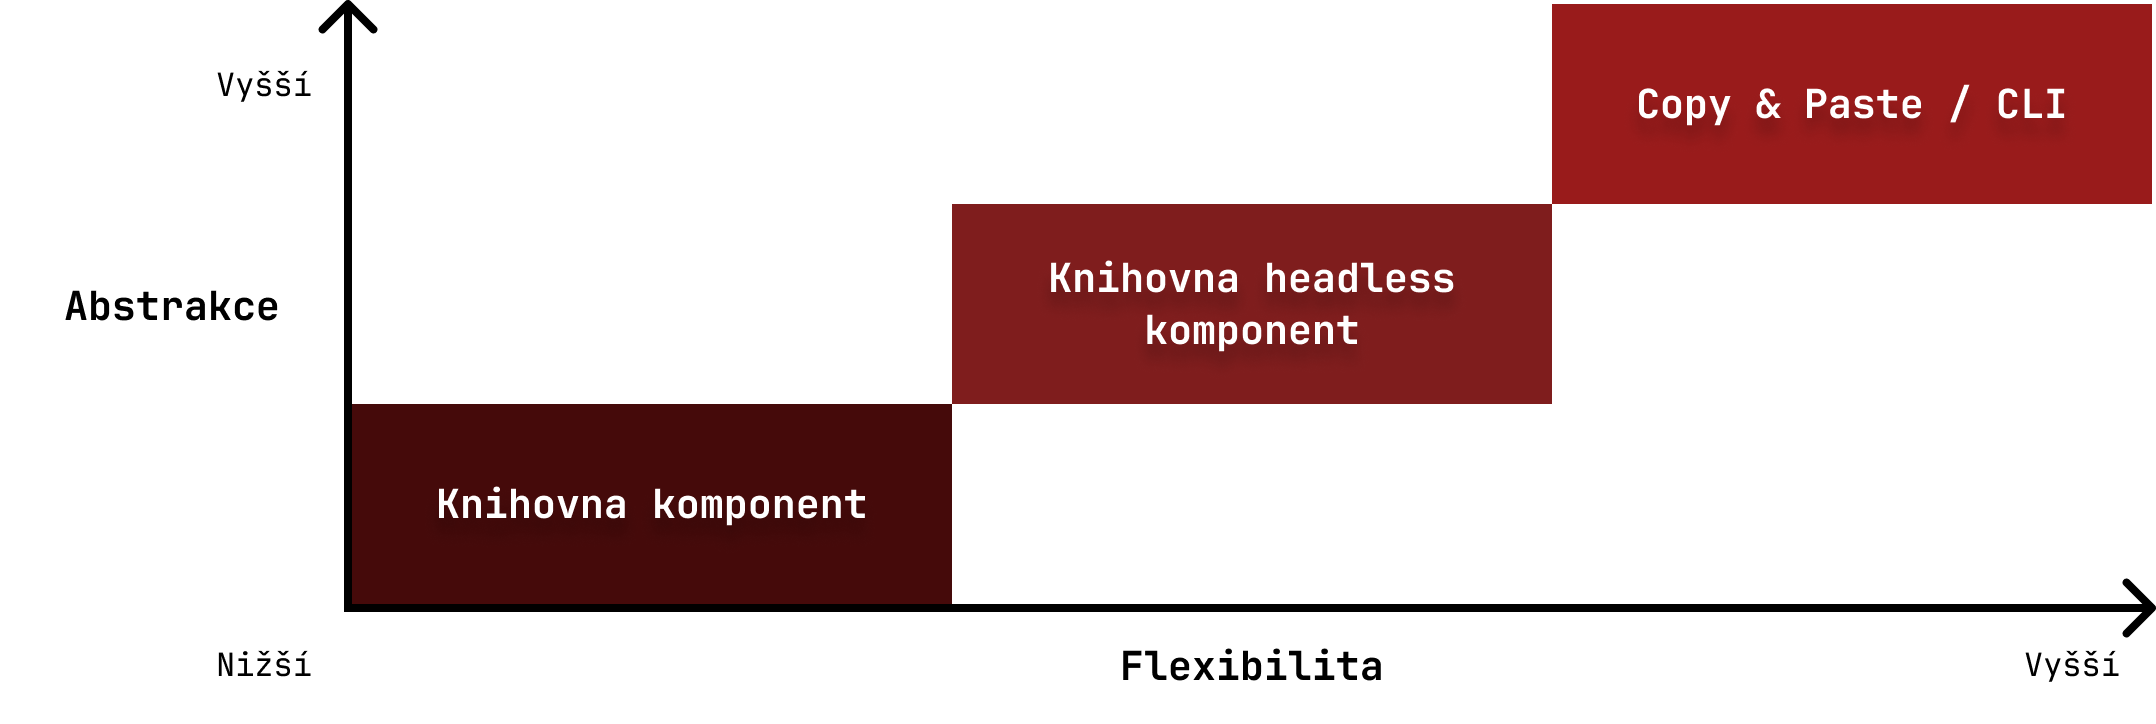
\includegraphics[width=\textwidth]{./assets/figures/component-lib-distribution-comparison.png}
      \captionsetup{justification=centering}
      \caption{Diagram abstrakce a flexibility různých přístupu k distribuci komponent}
      \label{component-lib-distribution-comparison}
\end{figure}

\section{Astro}

Vybranou technologií pro vytvoření dokumentace je \fr{Starlight}\footnote{\url{https://starlight.astro.build}} template postavený nad \fr{Astro}\footnote{\url{https://astro.build}} knihovnou.
Astro je \gls{ssg}, který používá vlastní syntaxi pro vytváření komponent.
Velkou výhodou je, že Astro umožňuje vnořit komponenty z jiných frameworků (React, Vue, Solid.js, Svelte a další) do Astro komponent bez použití \textit{iframe}.
Tento mechanismus lze použít pro vložení příkladové implementace komponenty přímo na stránku s dokumentací a zjednodušit tak uživatelům pochopení a účel komponenty.

Další důvod pro výběr Astro knihovny je možnost použití \fr{MDX}\footnote{\url{https://mdxjs.com}} syntaxe pro psaní dokumentace, která kombinuje markdown syntaxi s \gls{jsx}.

\section{Závěr kapitoly}

Tato kapitola popsala nejdůležitější technologie a přístupy, které jsou využity v rámci této práce.
Plná funkčnost celého projektu je závislá na dalších důležitých technologiích, které zde nejsou popsány neboť nejsou přímo relevantní k problematice tvorby znovupoužitelných komponent.

Samotná knihovna bude psána metodou primitiv, tedy funkcí v Solid.js, které vrací \gls{apg} logiku jako \textbf{props}, \textbf{state} a \textbf{reference} (viz kapitola~\ref{sec:structure}).
Taková knihovna může poté sloužit jako základ pro tvorbu designových systémů a (headless) knihoven komponent.

Solid.js knihovnu jsem zvolil ze dvou důvodů:

\begin{enumerate}
      \item Její ekosystém knihoven je stále v raných fázích a podobná knihovna respektive její části zde chybí.
      \item Knihovna solid.js má jisté vlastnosti, které ji odlišují od ostatních knihoven.
            Její reaktivní model je unikátní a přináší obrovské výhody z hlediska \textit{performance} na webu.
            Tato knihovna má potenciál optimalizovat a zlepšit uživatelská rozhraní.
\end{enumerate}

TypeScript je velice důležitý pro nové knihovny, neboť usnadňuje budoucí údržbu kódu a vývojářskou přívětivost.
Ve světě webového vývoje je TypeScript dnes už téměř standardem a jeho nepoužití by vedlo k výrazně snížené adopci knihovny komunitou vývojářů~\cite{stateofjs-2022}.


\part{Rešerše a analýza}

\chapter{Rešerše existujících řešení}

Tato kapitola rozebírá existující řešení v rámci JavaScriptového ekosystému.
Vyskytuje se tu bližší pohled na existující řešení pro React a Svelte protože hodně knihoven ve Solid.js z nich vychází.
Následně se rozebírá Solid.js a jeho chybějící části v rámci ekosystému.

\section{React}

React má obrovské zastoupení v rámci JavaScriptového ekosystému, proto kvalita knihoven zde bude vysoká díky velkému množství vývojářů a času věnovanému vývoji v této oblasti.

\subsection{React Aria}

React Aria\footnote{\url{https://react-spectrum.adobe.com/react-aria}} je open-source projekt od společnosti Adobe, který obsahuje velice robustní sadu primitiv v podobě React hooks.
Obsahuje velké množství komponent a interakcí, od nejzákladnějších jako jsou tlačítka, formulářové prvky až po složitější komponenty jako kalendáře.
Knihovna je velice dobře dokumentovaná a podporována komunitou.
Zároveň je distribuovaná bez stylů, proto je vhodná pro využití v rámci designových systémů.

\begin{table}[ht]
    \begin{ctucolortab}
        \begin{tabularx}{\textwidth}{Y Y}
            \bfseries \textcolor{OK}{Výhody} & \bfseries \textcolor{NOT_OK}{Nevýhody} \\\Midrule{}
            Flexibilita použití              & Vyšší nároky na udržování              \\
            Rozmanitost komponent            & ---
        \end{tabularx}
    \end{ctucolortab}
    \caption{Shrnutí výhod a nevýhod knihovny React Aria}
\end{table}

\subsection{Radix UI}

Radix UI\footnote{\url{https://radix-ui.com}} je knihovna komponent, která je zároveň postavená nad Radix UI primitives.
Radix primitives využívá na pozadí headless komponent, ačkoliv by název mohl evokovat opak.

To je zásadní rozdíl oproti React Aria, kde jsou komponenty vytvořené pomocí primitives.

\begin{table}[ht]
    \begin{ctucolortab}
        \begin{tabularx}{\textwidth}{Y Y}
            \bfseries \textcolor{OK}{Výhody} & \bfseries \textcolor{NOT_OK}{Nevýhody} \\\Midrule{}
            Jednoduchost použití             & Vyšší nároky na udržování              \\
            ---                              & Nižší rozmanitost komponent
        \end{tabularx}
    \end{ctucolortab}
    \caption{Shrnutí výhod a nevýhod knihovny Radix UI}
\end{table}

\subsection{Shadcn UI}

Shadcn UI\footnote{\url{https://ui.shadcn.com}} je copy and paste knihovna.
Z dokumentace nebo \gls{cli} dostupného skrze npm je možné nakopírovat předpis komponenty do uživatelem vybraného projektu.
Hodně komponent je založeno na Radix UI primitives.

\begin{table}[ht]
    \begin{ctucolortab}
        \begin{tabularx}{\textwidth}{Y Y}
            \bfseries \textcolor{OK}{Výhody} & \bfseries \textcolor{NOT_OK}{Nevýhody}         \\\Midrule{}
            Jednoduchost použití             & Flexibilita je závislá na použitých knihovnách \\
            Možnost upravit zdrojový kód     & ---
        \end{tabularx}
    \end{ctucolortab}
    \caption{Shrnutí výhod a nevýhod Shadcn UI}
\end{table}

\section{Svelte}

Svelte je novější framework, který se ubírá cestou nejvyššího komfortu pro vývojáře.
Rozhodl jsem se provést rešerši v rámci tohoto frameworku, protože Solid.js i Svelte používají reaktivní model změn.

\subsection{Melt UI}

Podobně jako React Aria je Melt UI\footnote{\url{https://melt-ui.com}} knihovna primitiv, v kontextu této knihovny se primitiva nazývají ``builders''.
Uživatelé konzumují tyto primitiva vytváří si tak komponenty s vlastní \gls{html} strukturou.
Z toho plyne, že je knihovna velice flexibilní na používání, ale zároveň je tak zvýšená náročnost na udržování komponent.
Výhodou je, že je možnost zde vytvořit příkladové použití těchto primitiv včetně základních stylů a usnadnit tak konzumentům práci.

\begin{table}[ht]
    \begin{ctucolortab}
        \begin{tabularx}{\textwidth}{Y Y}
            \bfseries \textcolor{OK}{Výhody} & \bfseries \textcolor{NOT_OK}{Nevýhody} \\\Midrule{}
            Vysoká flexibilita použití       & Vyšší nároky na udržování
        \end{tabularx}
    \end{ctucolortab}
    \caption{Shrnutí výhod a nevýhod knihovny Melt UI}
\end{table}

\section{Solid.js}
\label{sec:solid}

Solid.js je knihovna použitá v rámci této práce, proto je důležité provést rešerši a určit tak chybějící komponenty v rámci ekosystému.
Případně zjistit, zda lze navázat na práci již existujících knihoven.

\subsection{Solid Aria}

Solid Aria\footnote{\url{https://github.com/solidjs-community/solid-aria}} je port React Aria do Solid.js ekosystému podporovaný komunitou.
Bohužel vývoj zde již není příliš aktivní, protože na rozdíl od React Aria tento projekt není sponzorovaný větší společností.
Nicméně je zde možnost navázat na práci komunity a pokračovat v rozvoji této knihovny.

Velkou výhodou je, že port React kódu do Solid.js je na hodně místech velice podobný, proto je možné využít pokrok na samotné React Aria knihovně i zde.

\begin{table}[ht]
    \begin{ctucolortab}
        \begin{tabularx}{\textwidth}{Y Y}
            \bfseries \textcolor{OK}{Výhody} & \bfseries \textcolor{NOT_OK}{Nevýhody} \\\Midrule{}
            Flexibilita použití              & Neaktivní vývoj                        \\
            ---                              & Chybějící základní komponenty
        \end{tabularx}
    \end{ctucolortab}
    \caption{Shrnutí výhod a nevýhod Solid Aria}
\end{table}

\subsection{Kobalte}

Kobalte\footnote{\url{https://kobalte.dev}} je UI toolkit pro Solid.js, který obsahuje headless komponenty.
Hodně práce na Kobalte vychází ze Solid Aria, protože minimálně jeden z hlavních vývojářů Kobalte hojně pracoval i na Solid Aria.

\begin{table}[ht]
    \begin{ctucolortab}
        \begin{tabularx}{\textwidth}{Y Y}
            \bfseries \textcolor{OK}{Výhody} & \bfseries \textcolor{NOT_OK}{Nevýhody} \\\Midrule{}
            Jednoduchost použití             & Nižší flexibilita
        \end{tabularx}
    \end{ctucolortab}
    \caption{Shrnutí výhod a nevýhod knihovny Radix UI}
\end{table}

\section{Závěr rešerše}

Z rešerše vyplynulo, že ekosystém okolo Solid.js obsahuje několik knihoven, které řeší problematiku znovupoužitelných, přístupných komponent.
Další kapitola se zaměří na analýzu chybějících komponent z \gls{apg} návrhových vzorů a zda je možné navázat na práci již existujícího řešení.

\chapter{Analýza existujících řešení}

Tato kapitola rozebírá existující řešení v rámci JavaScriptového ekosystému.
Nejdříve rozeberu existující řešení pro React, protože hodně knihoven ve Solid.js z nich vychází.
Následně se podívám na Solid.js a rozeberu chybějící části v rámci jeho ekosystému.

\section{React}

\subsection{react-aria}

React aria je open-source projekt od společnosti Adobe, který obsahuje velice robustní sadu komponent a primitiv v podobě React hooks.
Obsahuje velké množství komponent a interakcí, od nejzákladnějších jako jsou tlačítka, formulářové prvky až po složitější komponenty jako kalendáře.
Knihovna je velice dobře dokumentovaná a podporována komunitou.
Zároveň je distribuovaná bez stylů, tedy se hodí pro využití v rámci designových systémů.

\begin{table}[ht]
    \begin{ctucolortab}
        \begin{tabularx}{\textwidth}{Y Y}
            \bfseries \textcolor{OK}{Výhody} & \bfseries \textcolor{NOT_OK}{Nevýhody} \\\Midrule{}
            Flexibilita použití              & Větší úsilí na udržování               \\
            Rozmanitost komponent
        \end{tabularx}
    \end{ctucolortab}
    \caption{Shrnutí výhod a nevýhod knihovny react-aria}
\end{table}

% \subsection{Radix UI}

% TODO

% \begin{table}[ht]
%     \begin{ctucolortab}
%         \begin{tabularx}{\textwidth}{Y Y}
%             \bfseries \textcolor{OK}{Výhody} & \bfseries \textcolor{NOT_OK}{Nevýhody} \\\Midrule{}
%             TODO                             & TODO                                   \\
%             TODO                             & TODO
%         \end{tabularx}
%     \end{ctucolortab}
%     \caption{Shrnutí výhod a nevýhod knihovny Radix UI}
% \end{table}

% \subsection{Shadcn UI}

% TODO

% \begin{table}[ht]
%     \begin{ctucolortab}
%         \begin{tabularx}{\textwidth}{Y Y}
%             \bfseries \textcolor{OK}{Výhody} & \bfseries \textcolor{NOT_OK}{Nevýhody} \\\Midrule{}
%             TODO                             & TODO                                   \\
%             TODO                             & TODO
%         \end{tabularx}
%     \end{ctucolortab}
%     \caption{Shrnutí výhod a nevýhod Shadcn UI}
% \end{table}

% \subsection{Headless UI}

% TODO

% \begin{table}[ht]
%     \begin{ctucolortab}
%         \begin{tabularx}{\textwidth}{Y Y}
%             \bfseries \textcolor{OK}{Výhody} & \bfseries \textcolor{NOT_OK}{Nevýhody} \\\Midrule{}
%             TODO                             & TODO                                   \\
%             TODO                             & TODO
%         \end{tabularx}
%     \end{ctucolortab}
%     \caption{Shrnutí výhod a nevýhod knihovny Headless UI}
% \end{table}

\clearpage

\section{Svelte}

\subsection{Melt UI}

Podobně jako react-aria je Melt UI knihovna primitiv, v kontextu této knihovny se primitiva nazývají ``builders''.
Uživatelé konzumují tyto primitiva vytváří si tak komponenty s vlastní HTML strukturou.
Z toho plyne, že je knihovna velice flexibilní na používání, ale zároveň je tak zvýšená náročnost na udržování komponent.
Výhodou je, že je možnost zde vytvořit příkladové použití těchto primitiv včetně základních stylů a usnadnit tak konzumentům práci.

\begin{table}[ht]
    \begin{ctucolortab}
        \begin{tabularx}{\textwidth}{Y Y}
            \bfseries \textcolor{OK}{Výhody} & \bfseries \textcolor{NOT_OK}{Nevýhody} \\\Midrule{}
            Vysoká flexibilita použití       & Vyšší nároky na udržování
        \end{tabularx}
    \end{ctucolortab}
    \caption{Shrnutí výhod a nevýhod knihovny Melt UI}
\end{table}

% \subsection{Svelte Headless UI}

% TODO

% \begin{table}[ht]
%     \begin{ctucolortab}
%         \begin{tabularx}{\textwidth}{Y Y}
%             \bfseries \textcolor{OK}{Výhody} & \bfseries \textcolor{NOT_OK}{Nevýhody} \\\Midrule{}
%             TODO                             & TODO                                   \\
%             TODO                             & TODO
%         \end{tabularx}
%     \end{ctucolortab}
%     \caption{Shrnutí výhod a nevýhod knihovny Svelte Headless UI}
% \end{table}


\part{Návrh a implementace}

\chapter{Návrh a struktura}

Tato kapitola popisuje strukturu repozitáře projektu a návrh implementace.

\section{Repozitář}

Samotný repozitář je tzv. monorepozitář, tedy repozitář s vícero projekty spravovanými pomocí balíčkovacího manažeru.
Pro tento projekt jsem zvolil balíčkovací nástroj pnpm, který má skvělou podporu pro monorepozitáře a šetří místo na disku pomocí pevných odkazů.

Níže je výčet všech projektů v rámi repozitáře:

% TODO: SSR hodit do akronymu.

\begin{itemize}
    \item \textbf{./packages/svelte-apg} je SvelteKit aplikace s využitím exportu komponent do balíčku, zde se nachází naimplementované komponenty. Zároveň tento projekt obsahuje i Storybook.
    \item \textbf{./projects/docs} je dokumentace pomocí Astro starlight template, zde je užitečný popis a ukázky využití komponent.
    \item \textbf{./projects/sveltekit-demo} je prázdná SvelteKit aplikace pro testování komponent v praktické aplikaci.
    \item \textbf{./projects/astro-demo} je prázdná Astro aplikace se Svelte pluginem, pro testování komponent v rámci island architektury.
\end{itemize}

% \subsection{Svelte APG}

% .

% \subsection{Dokumentace}

% .

\chapter{Implementace komponent}

Tato kapitola popisuje implementanční detaily komponent od samotného repozitáře po jejich distribuci.

\section{Repozitář}

Samotný repozitář je tzv. monorepozitář, tedy repozitář s vícero projekty spravovanými pomocí balíčkovacího manažeru.
Pro tento projekt jsem zvolil balíčkovací nástroj pnpm, který má skvělou podporu pro monorepozitáře a šetří místo na disku pomocí pevných odkazů.

Níže je výčet všech projektů v rámi repozitáře:

% TODO: SSR hodit do akronymu.

\begin{itemize}
    \item \textbf{./packages/svelte-apg} je SvelteKit aplikace s využitím exportu komponent do balíčku, zde se nachází naimplementované komponenty. Zároveň tento projekt obsahuje i Storybook.
    \item \textbf{./projects/docs} je dokumentace pomocí Astro starlight template, zde je užitečný popis a ukázky využití komponent.
    \item \textbf{./projects/sveltekit-demo} je prázdná SvelteKit aplikace pro testování komponent v praktické aplikaci.
    \item \textbf{./projects/astro-demo} je prázdná Astro aplikace se Svelte pluginem, pro testování komponent v rámci island architektury.
\end{itemize}

\subsection{Svelte APG}

.

\subsection{Dokumentace}

.


\part{Testování}

TODO

\section{Unit testing}

TODO

\chapter{Závěr}

TODO

\section{Budoucí vývoj}

TODO

\appendix

\printbibliography[title={Seznam literatury}]

\section{Literatura --- Přístupnost}

\printbibliography[keyword={a11y},heading=none]

\chapter{Obrázky}

\begin{landscape}
    \begin{figure}[p]
        \centering
        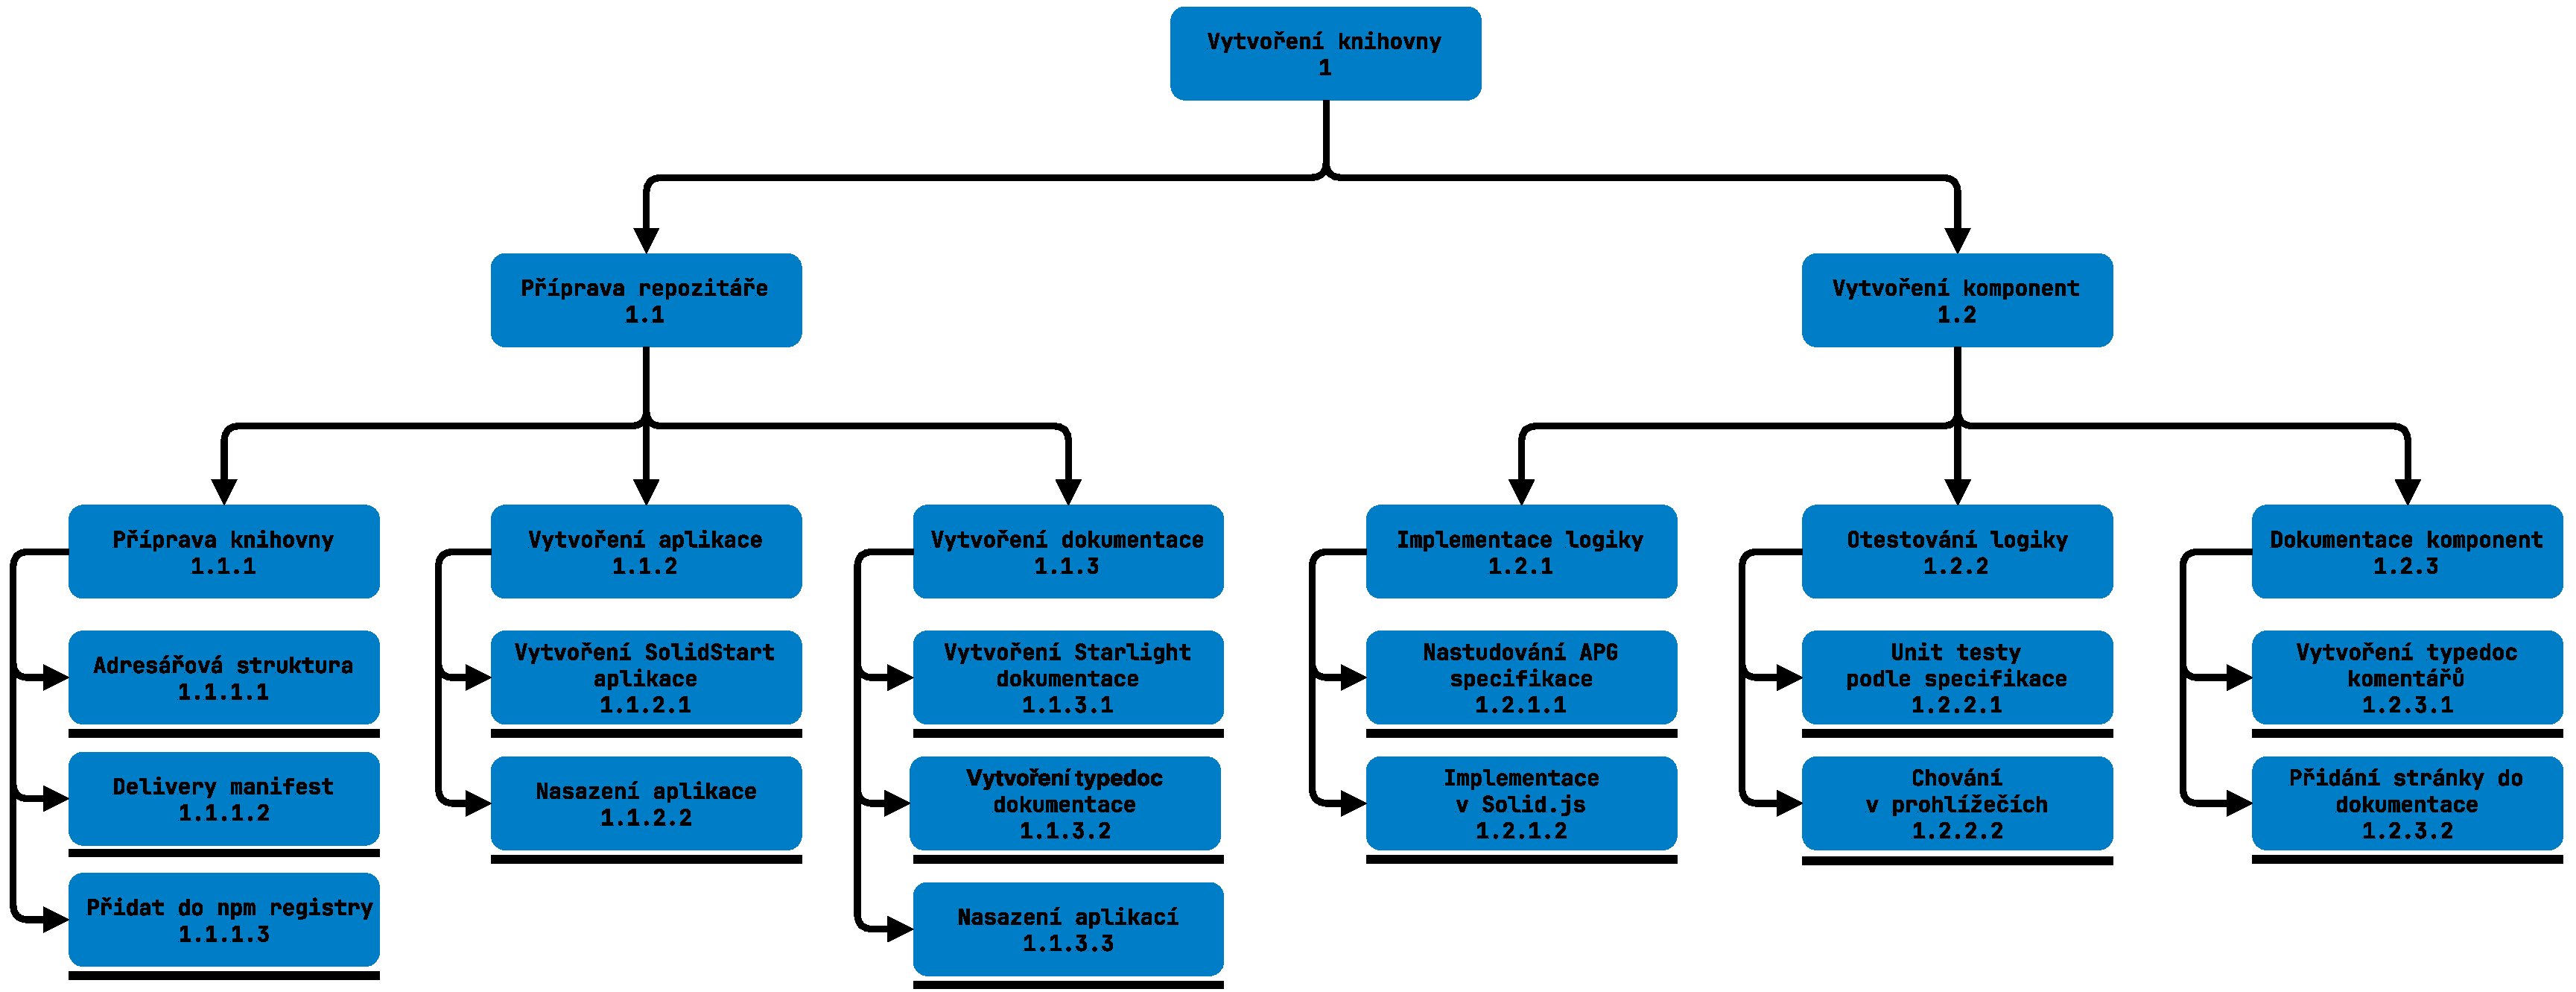
\includegraphics[max size={\linewidth}{\textheight}]{./assets/figures/hta-diagram.pdf}
        \captionsetup{justification=centering}
        \caption[HTA diagram vývoje knihovny]{HTA diagram (diagram autora)}
        \label{fig:hta}
    \end{figure}
\end{landscape}


\chapter{Tabulky}

\begin{table}[ht]
    \begin{tabularx}{\textwidth}{Y Y Y Y}\label{tab:implemented-components}
        \bfseries{Komponenta} & \bfseries{Solid Aria} & \bfseries{Kobalte} & \bfseries{Existence v ekosystému} \\\Midrule{}
        Accordion             & Ano                   & Ano                & Ano                               \\
        Alert                 & ---                   & Ano                & Ano                               \\
        Breadcrumb            & Ano                   & Ano                & Ano                               \\
        Button                & Ano                   & Ano                & Ano                               \\
        \textbf{Carousel}     & ---                   & ---                & \textbf{Ne}                       \\
        Checkbox              & Ano                   & Ano                & Ano                               \\
        Combobox              & ---                   & Ano                & Ano                               \\
        Dialog                & Ano                   & Ano                & Ano                               \\
        Disclosure            & ---                   & (Collapsible)      & Ano                               \\
        \textbf{Feed}         & ---                   & ---                & \textbf{Ne}                       \\
        \textbf{Grid}         & ---                   & ---                & \textbf{Ne}                       \\
        Listbox               & Ano                   & (Select)           & Ano                               \\
        Menu                  & Ano                   & Ano                & Ano                               \\
        Menubar               & ---                   & Ano                & Ano                               \\
        Meter                 & Ano                   & (Progress)         & Ano                               \\
        Radio Group           & Ano                   & Ano                & Ano                               \\
        Slider                & ---                   & Ano                & Ano                               \\
        SpinButton            & ---                   & (NumberField)      & Ano                               \\
        Switch                & Ano                   & Ano                & Ano                               \\
        \textbf{Toolbar}      & ---                   & ---                & \textbf{Ne}                       \\
        Tabs                  & Ano                   & ---                & Ano                               \\
        Tooltip               & ---                   & Ano                & Ano                               \\
        Tree View             & Ano                   & ---                & Ano                               \\
        \textbf{Treegrid}     & ---                   & ---                & \textbf{Ne}
    \end{tabularx}
    \caption{Tabulka implementovaných komponent v Solid.js ekosystému}
\end{table}


\chapter{Zdrojový kód}

TODO

\chapter{Odkazy}

\begin{itemize}
    \item \textbf{Dokumentace}

          \url{https://solid-apg-docs.vercel.app}
    \item \textbf{Zdrojový kód na GitHubu}

          \url{https://github.com/susickypavel/solid-apg}
    \item \textbf{Demo aplikace}

          \url{https://solid-apg-app.vercel.app}

    \item \textbf{Typedoc dokumentace}

          \url{https://solid-apg-typedoc.vercel.app}
\end{itemize}

\end{document}
